\newcommand{\figurescaling}{0.7}
\documentclass[a4paper,oneside,parskip=half]{scrartcl}

\usepackage{graphicx}
\usepackage{natbib}
\usepackage[utf8]{inputenc}
\usepackage{tabularx}
\usepackage{hyperref}
\usepackage{color}
\usepackage[usenames,dvipsnames,svgnames,table]{xcolor}
\usepackage{longtable}
\usepackage{slashbox}
\usepackage{multirow}
\usepackage{minibox}
\usepackage{placeins }
\usepackage{booktabs}
\usepackage[UKenglish]{babel}
\usepackage[T1]{fontenc}
\usepackage{lmodern}
\usepackage{pifont}
\usepackage{paralist}
\usepackage{listings}
\usepackage{enumitem}
\usepackage{multicol}
\usepackage[utf8]{inputenc}
\usepackage{authblk}

\title{Machine Learning WS2013}
\subtitle{Assignment 3 \\[0.8cm] {\rmfamily\normalfont\Large}}

\author[1]{Dino Rossegger}
\author[2]{Navid Rekabsaz}
\author[3]{Soroosh Mortezapoor}
\affil[1]{e0926471@student.tuwien.ac.at}
\affil[2]{e1129057@student.tuwien.ac.at}
\affil[3]{soroosh.mortezapoor@student.tuwien.ac.at}

\lstset{language=java,basicstyle=\ttfamily\footnotesize}

\begin{document}

\maketitle
\begin{abstract}
\end{abstract}

\section{Task}
The task was to analyse the differences in different feature selection techniques, i.e. analyse the difference in the selected features of the techniques. Therefore a java program had to be developed using the weka library to run the feature selection techniques on different datasets supplied by the lectors.

Furthermore a comparison of the results of k-nn using the top $n$ features of each feature selection technique and using mutual features was to be done. This was also implemented in the program using weka.

\section{Program Usage}
The java program uses ant to allow easy building and running of the program. In the build file the two properties \lstinline$weka.dir$ and \lstinline$lib.dir$ (containing apache commons cli) need to be changed.
Afterwards the program can be compiled using \lstinline$ant compile$, it is suggested to create a jar file using \lstinline$ant jar$.

The program accepts a number of arguments, in Listing~\ref{list:helpoutput} the help output can be seen. The only obligatory flag is \lstinline$-d <directory>$, specifying the directory from which the instances should be read. The rest of the arguments are optional, the help output in Listing~\ref{list:helpoutput} should be enough aid in understanding the usage of the program.
\begin{lstlisting}[caption=help output of the program, label=list:helpoutput]
 -c               compare results and find mutual features of result files
                   inside a directory
 -d <directory>   directory with instancefiles in csv or arff format
 -f <technique>   use specified feature selection technique
 -h               display this usage information
 -l               list all available feature selection techniques
 -n <n>           use top <n> attributes, default: 10
 -t <f>           consider attributes appearing in f per cent of the
                   result sets, default: 0.5

\end{lstlisting}
First the specified techniques (or all implemented techniques if \lstinline$-f$ is not set) are applied to the datasets, then the selected attributes are compared. At last a classifier is run using the features obtained from the feature selection methods. The precision, recall and f1-scores of the runs are printed on standard output.

\section{Technique Comparison}
In this section, we describe applied techniques and compare their selected attributed in order to understand how (dis)similar different algorithms are.

Applied techniques are described in Table\ref{table:techniques}. As it is shown eight supervised as well as two unsupervised algorithms are developed and used.

Since both unsupervised methods (PCI and LSA) reduce the input data to another matrix, the final attributes in reduced
matrix are not comparable with input data. In the case of applying Ranker search method on any of unsupervised evaluators, the ranked attributes will be a sequence from one to the number of attributes. Therefore, we decided to focus more on behavior of supervised methods.

We apply program's algorithm comparison ($-c$ parameter) on the result of eight supervised algorithms. Using provided data, we understand the number of mutual attributes between each pair of algorithms. in order to apply clustering on the methods, distance matrix is created. In order to form the matrix, the number of mutual attributes for each pair are subtracted from $50$. The distance matrix of $GTZAN$ dataset is shown in Table\ref{table:distancematrix}.

In the next step, by using R the methods are clustered based on Hierarchal Clustering algorithm. The clustering results of four datasets are shown in Figure\ref{fig:clustering}.

Based on the diagrams, following results can be concluded:
\begin{itemize}
\item ChiSquaredAttribute and InfoGain tend to have very similar results.
\item Besides ChiSquaredAttribute and InfoGain, SymmetricalUncertAttribute is the most similar one to them.
\item ConsistencySubset has always the most different results in comparison to the others.
\item CfsSubset and ReliefFAttribute seems to be related in some cases.
\end{itemize}

\begin{table}[p]
\begin{center}
\begin{tabular}{|c|c|c|c|}
\hline Attribute Evaluator & Search Method & Supervised/Unsupervised & Parameter Name \\
\hline CfsSubset & GreedyStepwise & Supervised & cfs-greedy\\
\hline ChiSquaredAttribute & Ranker & Supervised & chis-ranker\\
\hline ConsistencySubset & BestFirst & Supervised & cons-bestfirst\\
\hline GainRatioAttribute & Ranker & Supervised & gainr-ranker\\
\hline InfoGain & Ranker & Supervised & ig-ranker\\
\hline OneRAttribute & Ranker & Supervised & oner-ranker\\
\hline ReliefFAttribute & Ranker & Supervised & rel-ranker\\
\hline SymmetricalUncertAttribute & Ranker & Supervised & sua-ranker\\
\hline PrincipalComponents & Ranker & Unsupervised & pca-ranker\\
\hline LatentSemanticAnalysis & Ranker & Unsupervised & lsa-ranker\\
\hline
\end{tabular}
\caption{Applied attribute selection techniques}
\label{table:techniques}
\end{center}
\end{table}


\begin{table}[p]
\begin{center}
\begin{tabular}{|c|p{1.3cm}|p{1.3cm}|p{1.3cm}|p{1.3cm}|p{1.3cm}|p{1.3cm}|p{1.3cm}|p{1.3cm}|}
\hline & cfs-greedy & chis-ranker & cons-bestfirst & gainr-ranker & ig-ranker & oner-ranker & rel-ranker & sua-ranker\\
\hline cfs-greedy & 0 & 41 & 46 & 44 & 40 & 39 & 28 & 40\\
\hline chis-ranker & 41 & 0 & 48 & 39 & 9 & 21 & 37 & 9\\
\hline cons-bestfirst & 46 & 48 & 0 & 50 & 48 & 49 & 47 & 49\\
\hline gainr-ranker & 44 & 39 & 50 & 0 & 37 & 34 & 41 & 34\\
\hline ig-ranker & 40 & 9 & 48 & 37 & 0 & 16 & 36 & 4\\
\hline oner-ranker & 39 & 21 & 49 & 34 & 16 & 0 & 37 & 16\\
\hline rel-ranker & 28 & 37 & 47 & 41 & 36 & 37 & 0 & 36\\
\hline sua-ranker & 40 & 9 & 49 & 34 & 4 & 16 & 36 & 0\\
\hline
\end{tabular}
\caption{Applied attribute selection techniques}
\label{table:distancematrix}
\end{center}
\end{table}


\begin{figure}[p]
\begin{center}
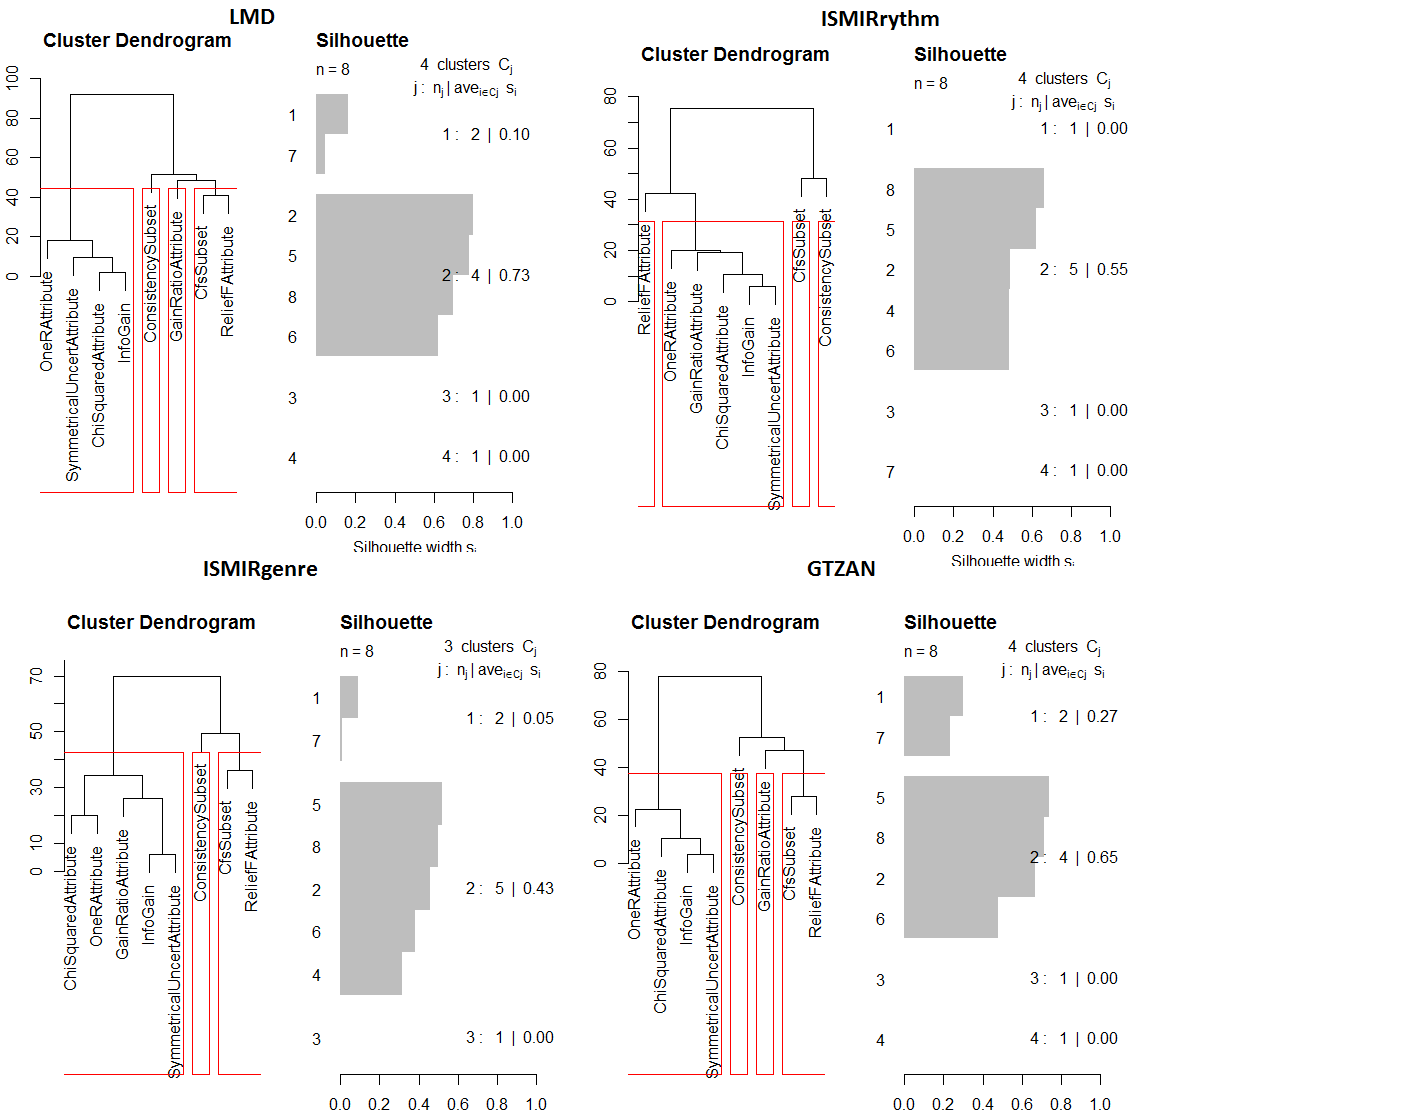
\includegraphics[scale=0.5]{fig/diagram_all.png}
\caption{Attribute selection methods clustering for four datasets
\label{fig:clustering}}
\end{center}
\end{figure}

\section{Comparison on Classifier}
Detailed results of running a $k-$nearest neighbors classifier on $4$ different
datasets, {\it GTZAN\_O.rp.arff}, {\it ISMIRgenre.rp.arff}, {\it
ISMIRrhythm.rp.arff} and {\it LMD.rp.arff} with different methods of attribute
selection are shown in Tables~\ref{table:classifier:GTZANO6} $\ldots$ \ref{table:classifier:LMD2}.

Tests are conducted in a way that all four datasets are used for attribute
selection with three different combination of attribute selector algorithms.
Once with a combination of \{ ChiSquaredAttribute, InfoGain,
SymmetricalUncertAttribute, ReliefFAttribute, OneRAttribute, GainRatioAttribute
\}, another time with \{ ChiSquaredAttribute, InfoGain,
SymmetricalUncertAttribute, ReliefFAttribute \} and finally with \{ChiSquaredAttribute, InfoGain,
SymmetricalUncertAttribute \}. 

In order to have train/test sets, each dataset is broken to $2$ subsets, one
containing $\frac{3}{4}$ of the data as train set and one with the rest
$\frac{1}{4}$ as a test set.

In each run, firstly each dataset is classified
without attribute selection and with all attributes it has. Subsequently, each
attribute selection method is used to find a subset of attributes, which in our
case, top most $50$ selected attributes are used to perform the
classification task and hereafter we call them single rounds. Finally, two
rounds, one with most appearing attributes in single rounds where here all
attributes appearing at least in half of the selected sets of attributes and another round with a union of top most $N$ selected attributes
from each single run are performed.

In Tables~\ref{table:classifier:GTZANO6} $\ldots$
\ref{table:classifier:LMD6}, gained results of all firstround, single rounds and
final rounds are shown. Tables~\ref{table:classifier:GTZANO3} $\ldots$
\ref{table:classifier:LMD3} also show the results of the final rounds for the
second run and subsequently, Tables~\ref{table:classifier:GTZANO2} $\ldots$
\ref{table:classifier:LMD2} represent the results of the final round for the
third run. $\searrow$ and $\nearrow$ indicate improvement or demotion of f-score
results of most appearing and union approaches.

As it is clear, except for one dataset, ISMIRgenre.rp.arff, in the first run,
which has a better result with the union of $N$ top most selected attributes in
single rounds, all other combination deliver worse results compared to the best
result of their single rounds.


\begin{table}[p]
\begin{center}
\begin{tabular}{|c|c|c|c|}
\hline Algorithm: & Precision: & Recall & F-Score\\
\hline Randomly chosen attributes & 0.02400 & 0.01200 & {\bf 0.01600}\\
\hline ChiSquaredAttribute-Ranker-Supervised & 0.00000 & 0.00000 & 0.00000\\
\hline InfoGain-Ranker-Supervised & 0.00000 & 0.00000 & 0.00000\\
\hline SymmetricalUncertAttribute-Ranker-Supervised & 0.00000 & 0.00000 &
0.00000\\
\hline ReliefFAttribute-Ranker-Supervised & 0.03333 & 0.00800 & 0.01290\\
\hline OneRAttribute-Ranker-Supervised & 0.00000 & 0.00000 & 0.00000\\
\hline GainRatioAttribute-Ranker-Supervised & 0.01250 & 0.00400 & 0.00606
\\
\hline Most appearing attributes & 0.00000 & 0.00000 & 0.00000 $\searrow$\\
\hline Union of selected Attributes & 0.00714 & 0.00400 & 0.00513 $\searrow$\\

\hline
\end{tabular}
\caption{Results for GTZAN\_O.rp.arff with 6 attribute selection methods}
\label{table:classifier:GTZANO6}
\end{center}
\end{table}



\begin{table}[p]
\begin{center}
\begin{tabular}{|c|c|c|c|}
\hline Algorithm: & Precision: & Recall & F-Score\\
\hline Randomly chosen attributes & 0.96661 & 0.70959 & 0.79623\\
\hline ChiSquaredAttribute-Ranker-Supervised & 0.69863 & 0.00000 & 0.80376\\
\hline InfoGain-Ranker-Supervised & 0.98497 & 0.66027 & 0.77380\\
\hline SymmetricalUncertAttribute-Ranker-Supervised & 0.98084 & 0.76271 &
0.76271\\
\hline ReliefFAttribute-Ranker-Supervised & 0.98636 & 0.70137 & {\bf 0.80834}\\
\hline OneRAttribute-Ranker-Supervised & 0.98690 & 0.70137 & 0.79764\\
\hline GainRatioAttribute-Ranker-Supervised & 0.98017 & 0.68219 & 0.77885\\
\hline Most appearing attributes & 0.98122 & 0.67123 & 0.77661 $\searrow$\\
\hline Union of selected Attributes & 0.96026 & 0.73151 & 0.82033 $\nearrow$\\

\hline
\end{tabular}
\caption{Results for ISMIRgenre.rp.arff with 6 attribute selection methods}
\label{table:classifier:ISMIRgenre6}
\end{center}
\end{table}



\begin{table}[p]
\begin{center}
\begin{tabular}{|c|c|c|c|}
\hline Algorithm: & Precision: & Recall & F-Score\\
\hline Randomly chosen attributes & 0.75446 & 0.12000 & 0.19154\\
\hline ChiSquaredAttribute-Ranker-Supervised & 0.09714 & 0.00000 & 0.17239\\
\hline InfoGain-Ranker-Supervised & 0.82679 & 0.13143 & {\bf 0.22677}\\
\hline SymmetricalUncertAttribute-Ranker-Supervised & 0.85219 & 0.11429 &
0.20109\\
\hline ReliefFAttribute-Ranker-Supervised & 0.55143 & 0.06286 & 0.11066\\
\hline OneRAttribute-Ranker-Supervised & 0.92082 & 0.11429 & 0.19961\\
\hline GainRatioAttribute-Ranker-Supervised & 0.76245 & 0.11429 & 0.19437\\
\hline Most appearing attributes & 0.82945 & 0.12000 & 0.20956 $\searrow$\\
\hline Union of selected Attributes & 0.45543 & 0.03429 & 0.06247 $\searrow$\\

\hline
\end{tabular}
\caption{Results for ISMIRrhythm.rp.arff with 6 attribute selection methods}
\label{table:classifier:ISMIRrhythm6}
\end{center}
\end{table}


\begin{table}[p]
\begin{center}
\begin{tabular}{|c|c|c|c|}
\hline Algorithm: & Precision: & Recall & F-Score\\
\hline Randomly chosen attributes & 0.10211 & 0.09181 & 0.07886\\
\hline ChiSquaredAttribute-Ranker-Supervised & 0.07281 & 0.09057 & 0.06168\\
\hline InfoGain-Ranker-Supervised & 0.06634 & 0.08437 & 0.05483\\
\hline SymmetricalUncertAttribute-Ranker-Supervised & 0.06634 & 0.09926 &
0.07051\\
\hline ReliefFAttribute-Ranker-Supervised & 0.13408 & 0.10174 & {\bf 0.10043}\\
\hline OneRAttribute-Ranker-Supervised & 0.07558 & 0.08561 & 0.05833\\
\hline GainRatioAttribute-Ranker-Supervised & 0.06802 & 0.09801 & 0.06907\\
\hline Most appearing attributes & 0.07239 & 0.08933 & 0.06056 $\searrow$\\
\hline Union of selected Attributes & 0.07349 & 0.08561 & 0.06733 $\searrow$\\

\hline
\end{tabular}
\caption{Results for LMD.rp.arff with 6 attribute selection methods}
\label{table:classifier:LMD6}
\end{center}
\end{table}





\begin{table}[p]
\begin{center}
\begin{tabular}{|c|c|c|c|}
\hline Algorithm: & Precision: & Recall & F-Score\\
\hline Most appearing attributes & 0.00000 & 0.00000 & 0.00000 $\searrow$\\
\hline Union of selected Attributes & 0.00667 & 0.00400 & 0.00500 $\searrow$\\

\hline
\end{tabular}
\caption{Results for GTZAN\_O.rp.arff with 3 attribute selection methods}
\label{table:classifier:GTZANO3}
\end{center}
\end{table}


\begin{table}[p]
\begin{center}
\begin{tabular}{|c|c|c|c|}
\hline Algorithm: & Precision: & Recall & F-Score\\
\hline Most appearing attributes & 0.98562 & 0.67945 & 0.78850 $\searrow$\\
\hline Union of selected Attributes & 0.96893 & 0.61644 & 0.74669 $\searrow$\\

\hline
\end{tabular}
\caption{Results for ISMIRgenre.rp.arff with 3 attribute selection methods}
\label{table:classifier:ISMIRgenre3}
\end{center}
\end{table}


\begin{table}[p]
\begin{center}
\begin{tabular}{|c|c|c|c|}
\hline Algorithm: & Precision: & Recall & F-Score\\
\hline Most appearing attributes & 0.81524 & 0.10857 & 0.19120 $\searrow$\\
\hline Union of selected Attributes & 0.44571 & 0.02286 & 0.04348 $\searrow$\\

\hline
\end{tabular}
\caption{Results for ISMIRrhythm.rp.arff with 3 attribute selection methods}
\label{table:classifier:ISMIRrhythm3}
\end{center}
\end{table}


\begin{table}[p]
\begin{center}
\begin{tabular}{|c|c|c|c|}
\hline Algorithm: & Precision: & Recall & F-Score\\
\hline Most appearing attributes & 0.07194 & 0.09057 & 0.06151 $\searrow$\\
\hline Union of selected Attributes & 0.08266 & 0.07940 & 0.06291 $\searrow$\\

\hline
\end{tabular}
\caption{Results for LMD.rp.arff with 3 attribute selection methods}
\label{table:classifier:LMD3}
\end{center}
\end{table}






\begin{table}[p]
\begin{center}
\begin{tabular}{|c|c|c|c|}
\hline Algorithm: & Precision: & Recall & F-Score\\
\hline Most appearing attributes & 0.00000 & 0.00000 & 0.00000 $\searrow$\\
\hline Union of selected Attributes & 0.00667 & 0.00400 & 0.00500 $\searrow$\\

\hline
\end{tabular}
\caption{Results for GTZAN\_O.rp.arff with 2 attribute selection methods}
\label{table:classifier:GTZANO2}
\end{center}
\end{table}


\begin{table}[p]
\begin{center}
\begin{tabular}{|c|c|c|c|}
\hline Algorithm: & Precision: & Recall & F-Score\\
\hline Most appearing attributes & 0.97608 & 0.69589 & 0.79594 $\searrow$\\
\hline Union of selected Attributes & 0.96861 & 0.61096 & 0.74280 $\searrow$\\

\hline
\end{tabular}
\caption{Results for ISMIRgenre.rp.arff with 2 attribute selection methods}
\label{table:classifier:ISMIRgenre2}
\end{center}
\end{table}


\begin{table}[p]
\begin{center}
\begin{tabular}{|c|c|c|c|}
\hline Algorithm: & Precision: & Recall & F-Score\\
\hline Most appearing attributes & 0.80204 & 0.10286 & 0.18210 $\searrow$\\
\hline Union of selected Attributes & 0.44571 & 0.01714 & 0.03302 $\searrow$\\

\hline
\end{tabular}
\caption{Results for ISMIRrhythm.rp.arff with 2 attribute selection methods}
\label{table:classifier:ISMIRrhythm2}
\end{center}
\end{table}


\begin{table}[p]
\begin{center}
\begin{tabular}{|c|c|c|c|}
\hline Algorithm: & Precision: & Recall & F-Score\\
\hline Most appearing attributes & 0.07055 & 0.08933 & 0.06012 $\searrow$\\
\hline Union of selected Attributes & 0.06551 & 0.06948 & 0.04955 $\searrow$\\

\hline
\end{tabular}
\caption{Results for LMD.rp.arff with 2 attribute selection methods}
\label{table:classifier:LMD2}
\end{center}
\end{table}


\end{document}
